\chapter{Unstructured uncertainty modeling and robustness}

\section{Unstructured uncertainty vs Structured uncertainty}
Regarding the physical aspect of uncertainty, irrespective of their complexity, mathematical models cannot exactly describe a real physical process. Sometimes, we may prefer simplified approximate models. Thus, model uncertainty has to be taken into account whne a mathematical model is used to analyze the behavior of a system to design a feedback control system.
\subsection{Source of model uncertainty}
The uncertainty in the mathematical models can stem from:
\begin{itemize}
    \item Intentional approximation of high-order or infinite-dimensional systems by low order models, e.g. neglected fast actuator and/or sensor dynamics.
    \item Neglected some or all high-frequency bending and torsional modes.
    \item Neglected far-away stable poles and/or far-away minimum and non-minimum phase zeros.
    \item Neglected small time delays (physical or computaitonal)
    \item Parameter uncertainty in coefficients of transefer functions 
    \item Neglected small non-linearities
\end{itemize}

\textbf{Model uncertainty is essentially due to:}
\begin{itemize}
    \item physical parameters not exactly known
    \item unmodeled (linear or nonlinear) dynamic
\end{itemize}

Uncertainty due to approximate knowledge of some parameter values is called \textbf{parameter uncertainty}\\
Uncertainty due to unmodeled dynamics is called \textbf{dynamic uncertainty}.\\

The basic approach to take uncertainty into account is to describe the plant under study as a member of a set of systems, also called \textbf{model set}. From now on, we will restrict our attention to LTI uncertain systems. Model sets for LTI uncertain systems can be classified as:
\begin{itemize}
    \item \textbf{Structured uncertainty model set}: when the set is parametrized by a finite number of parameters
    \item \textbf{Unstructured uncertainty model set}: when complete ignorance regarding the order and the phase behavior of the system is assumed.
\end{itemize}

\textbf{Parametric uncertainty} leads straightforwardly to \textbf{structured model sets}. It can also be described (with "some conservativeness") by means of \textbf{unstructured model sets.} \textbf{Dynamic uncertainty} leads straightforwardly to \textbf{unstructured model sets}.\\

Four different unstructured model sets will be considered, which will refer to:
\begin{itemize}
    \item additive uncertainty
    \item multiplicative uncertainty
    \item inverse additive uncertainty
    \item inverse multiplicative uncertainty
\end{itemize}
\begin{example}
In order to have an intuition about the set of models consider the following simple case:
\[
\alpha: 4\div8, \alpha \in \mathbb{R}
\]
Considering $\alpha_n$ as the nominal value of the parameter, we can consider the set of model $M$ as follow:
\[
M = \{\alpha: \alpha = \alpha_n + r\delta: \:\:\:\:\: |\delta| \leq 1; \: r = 2;\: \alpha = 6\}
\]
Here, the variable $r$ signifies the magnitude of the uncertainty. The larger $r$, the larger the uncertainty regarding the value of the parameter.
\end{example}

All in all, in order to model uncertainty in an unstructured manner, we should choose a nominal plant, and a weighting function $W_u$ quantifying the magnitude of uncertainty.

\subsection{The additive uncertainty model set}
The mathematical set of this kind of uncertainty model is as follows:
\[
M_a = \{G_p(s):\:G_p(s)\,=\,G_{pn}+W_u(s)\Delta(s),\,\|\Delta(s)\|_\infty\leq 1 \}
\]
where:$G_{pn}$ is the nominal model of the plant. $\Delta(s)$ can be any possible transfer function whose $H_\infty$ norm is less than 1. \textbf{$W_u(s)$ is weighting function which accounts for the size of the uncertainty}. 
\begin{QandAbox}
It is assumed that all systems belonging to $M_a$ must have the same number of unstable poles. 
\end{QandAbox}

\begin{figure}[H]
    \centering
    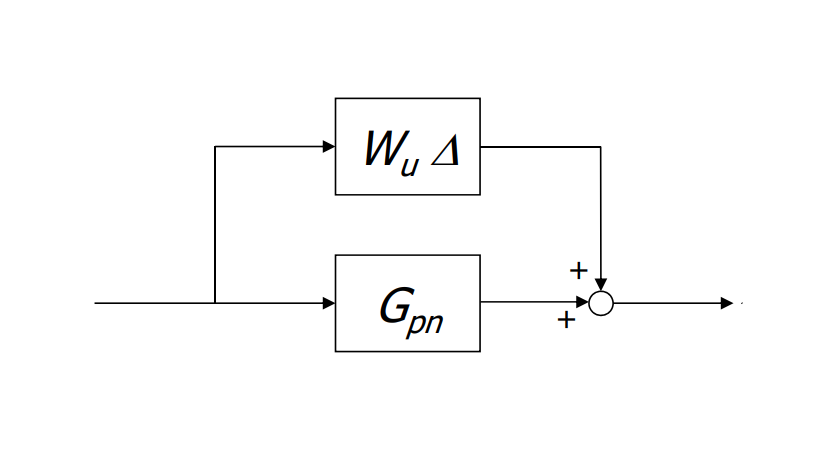
\includegraphics[width=0.5\textwidth]{additive-uncertainty.png}
    \caption{The block diagram description of additive uncertainties}
    \label{fig:sensitivity}
\end{figure}

\subsubsection{Use cases:}
\begin{enumerate}
    \item \textbf{Disturbances and External Noise Influences:}\\
    \textbf{Scenario:} When the system experiences external disturbances that add to its output directly (e.g., sensor noise, external forces, or environmental disturbances).\\
\textbf{Why Additive:} The uncertainty does not affect the system's internal dynamics but introduces variation at the output.\\
\textbf{Example:} A temperature sensor in a heating system where fluctuations in room temperature due to external drafts or minor noise in measurement affect the output but not the heater’s internal dynamics.
    \item \textbf{Low-Frequency Uncertainty Dominance:}\\
    \textbf{Scenario:} When uncertainty is mainly present at low frequencies, where it can dominate system behavior.\\
\textbf{Why Additive:} At low frequencies, the additive model is effective as it can capture steady-state or slow-moving disturbances, which are common in control applications.\\
\textbf{Example:} An aircraft with control surfaces that may experience slow, random wind gusts affecting the output position without impacting the fundamental control dynamics.
    \item \textbf{Unmodeled Dynamics Outside the Bandwidth of Interest:}\\
  \textbf{Scenario:} When there are unmodeled high-frequency dynamics that don’t impact the primary system response but could affect output measurements.\\
\textbf{Why Additive:} Additive uncertainty is often used to approximate unmodeled dynamics that are outside the control bandwidth but might still show up in system outputs.\\
\textbf{Example:} A robotic arm with minor high-frequency oscillations in its joints; while these oscillations are outside the primary control bandwidth, they are added as uncertainties in the output.
    \item \textbf{Unmodeled Dynamics Outside the Bandwidth of Interest:}\\
    \textbf{Scenario:} When there are unmodeled high-frequency dynamics that don’t impact the primary system response but could affect output measurements.\\
\textbf{Why Additive:} Additive uncertainty is often used to approximate unmodeled dynamics that are outside the control bandwidth but might still show up in system outputs.\\
\textbf{Example:} A robotic arm with minor high-frequency oscillations in its joints; while these oscillations are outside the primary control bandwidth, they are added as uncertainties in the output.
    \item \textbf{Measurement Uncertainties at System Output:}\\
   \textbf{ Scenario:} When the primary source of uncertainty arises from inaccuracies in measurement rather than the system's internal dynamics.\\
\textbf{Why Additive:} Measurement noise or sensor errors can often be well-represented by additive uncertainty since they appear at the output stage.\\
\textbf{Example:} In a feedback control system for temperature regulation, if the thermocouple sensor has random noise, this noise can be treated as an additive uncertainty.
\end{enumerate}

\begin{example}
consider a plant described by the following transfer function:
\[
G_p(s) = \frac{1}{\left( \frac{s}{5} + 1 \right) \left( \frac{s^2}{2500} + \frac{s}{2500} + 1 \right) \left( \frac{s^2}{6400} + \frac{1.6s}{6400} + 1 \right)}
\]
This is the transfer function of an electrical motor. The slowest pole correspond to the mechanical dynamic of the system. The other two poles which are faster, correspond to the electrical poles. Assume that in order to simplify the plant model to be used in controller design, we neglect the flexible modes. This is equivalent to chose thet following transfer function for nominal model:
\[
G_{pn}(s)=\frac{1}{(1+\frac{s}{5})}
\]
\textbf{In order ot descirbe the uncertainty due to the unmodelled dynamics which corresponds to the flexible modes, we considder and additive uncertainty model set.}
$G_p$ has one real pole and two pairs of lightly damped complex-conjugate poles (flexible modes). \\
Assume that in order to simplify the plant model to be used in the controller design, we neglect the flexible modes. This is equivalent to choose the following transfer function for the nominal model:\\
\[
G_{pn} = \frac{1}{\frac{s}{5}+1}
\]
\end{example}
In order to describe the uncertainty due to the unmodeled dynamics which corresponds to the flexible modes, we consider an additive uncertainty model set.
The following additive uncertainty model set is considered 
\[
M_a = \{G_p(s): G_p(s) = G_{pn} + W_u(s)\Delta(s), \|\Delta(s)\|\leq 1\}
\]
where, by construction, the weighting function $W_u$ must satisfy the following condition:
\[
\|\frac{G_p(s)-G_{pn}(s)}{W_u(s)}\|_\infty = \|\Delta(s)\|_\infty \leq 1
\]
which is equivalent to:
\[
|G_p(j\omega)-G_{pn}(j\omega)| \leq |W_u(j\omega)| \:\:\forall \omega
\]


\begin{figure}[H]
    \centering
    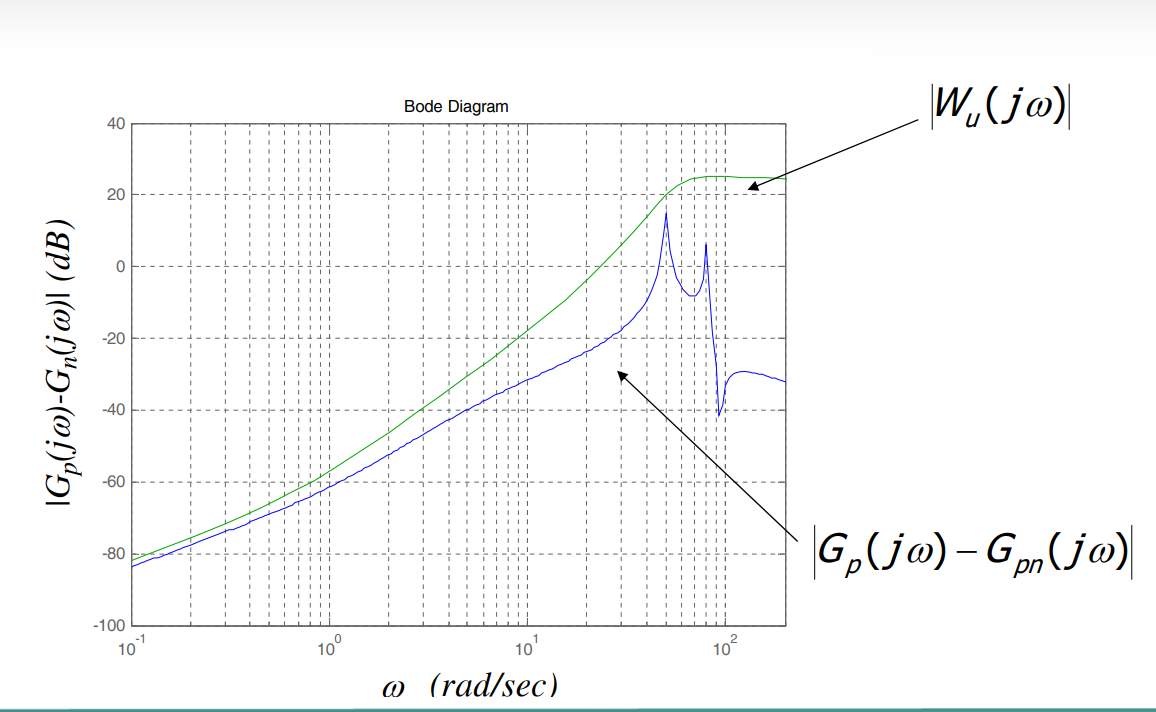
\includegraphics[width=0.75\textwidth]{additive-weighting.png}
    \caption{A possible weighting function describing the unstructured uncertainty that is modelled in an additive manner.}
\end{figure}

Pay attnetion that this weighting function should be as tight as possible in order to reduce the conservativeness.


\subsection{The multiplicative uncertainty model set}
The mathematical set of this kind of uncertainty model is as follows:
\[
M_m = \{G_p(s):\:G_p(s)\,=\,G_{pn}[1 + W_u(s)\Delta(s)],\,\|\Delta(s)\|_\infty\leq 1 \}
\]
where:$G_{pn}$ is the nominal model of the plant. $\Delta(s)$ can be any possible transfer function whose $H_\infty$ norm is less than 1. \textbf{$W_u(s)$ is weighting function which accounts for the size of the uncertainty}. 
\begin{QandAbox}
??It is assumed that all systems belonging to $M_m$ must have the same number of unstable poles. ?? Not written in the slides
\end{QandAbox}

\begin{figure}[H]
    \centering
    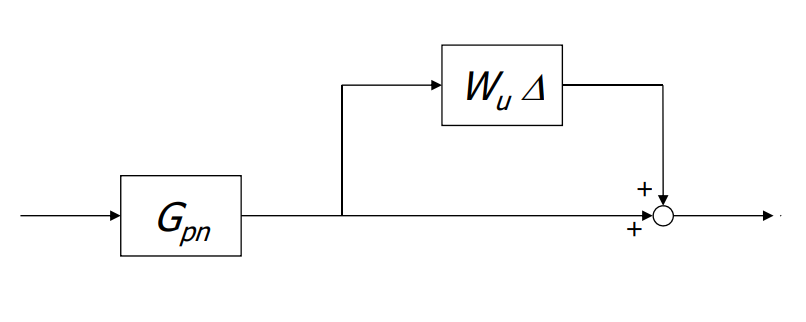
\includegraphics[width=0.5\textwidth]{multiplicative-uncertainty.png}
    \caption{The block diagram description of multiplicative uncertainty}
\end{figure}
Considering the formulation of the problem, the weighting function $W_u$ must satisfy the following condition:
\[
\|(\frac{G_p(s)}{G_{pn}}-1)\frac{1}{W_u(s))}\|_\infty = \|\Delta(s)\|_\infty \leq 1
\]
which is equivalent to:
\[
|(\frac{G_p(s)}{G_{pn}}-1)| \leq |W_u(j\omega)| \:\: \forall \omega
\]
here, $G_p$ represents the whole family.
\subsubsection{Use cases:}
\begin{enumerate}
    \item \textbf{Modeling Uncertainties in Plant Dynamics:}\\
    \textbf{Scenario:} When uncertainties arise directly in the plant's dynamics, affecting the system’s behavior multiplicatively (e.g., gain or phase variations).\\
    \textbf{Why Multiplicative:} The uncertainty scales with the nominal system dynamics, making multiplicative uncertainty ideal for capturing such variations.\\
    \textbf{Example:} In an electronic circuit, variations in component values (e.g., resistance, inductance) lead to changes in the system gain or frequency response, which are proportional to the nominal dynamics.

    \item \textbf{High-Frequency Uncertainty Dominance:}\\
    \textbf{Scenario:} When the system’s response at high frequencies is uncertain due to unmodeled dynamics or parameter variations.\\
    \textbf{Why Multiplicative:} At high frequencies, uncertainties often scale with the system's dynamics, as unmodeled dynamics or delays tend to affect system performance multiplicatively.\\
    \textbf{Example:} An aircraft experiencing structural flexibilities at high frequencies where these unmodeled dynamics alter the transfer function of the nominal model.

    \item \textbf{Frequency-Dependent Plant Gain Variations:}\\
    \textbf{Scenario:} When the gain or phase of the system varies with operating conditions or frequency.\\
    \textbf{Why Multiplicative:} Gain variations at specific frequencies are well-captured by scaling the nominal plant model by an uncertainty term.\\
    \textbf{Example:} A motor whose torque output depends on frequency, where small deviations in frequency lead to proportional changes in output gain.

    \item \textbf{Unmodeled Dynamics Near Control Bandwidth:}\\
    \textbf{Scenario:} When the primary concern is unmodeled dynamics near or within the system’s control bandwidth.\\
    \textbf{Why Multiplicative:} Unmodeled dynamics close to the system's natural frequency often affect the plant’s behavior in a manner proportional to its nominal transfer function.\\
    \textbf{Example:} A robotic arm where flexible joint dynamics close to the control bandwidth lead to uncertain oscillatory behaviors.

    \item \textbf{Process Variations in Gain or Time Delay:}\\
    \textbf{Scenario:} When physical parameters like gain or time delay are subject to process variations due to manufacturing tolerances or operational conditions.\\
    \textbf{Why Multiplicative:} Variations in these parameters influence the plant transfer function multiplicatively, altering both the magnitude and phase of the response.\\
    \textbf{Example:} A chemical reactor where temperature-dependent reactions cause the plant's time constants to vary proportionally with operating conditions.
\end{enumerate}

\begin{example}
Consider a plant described by the following transfer function
\[
G_p(s) = \frac{K}{s-2}
\]
where $K$ is an uncertain real constant which satisfies:
\[
5 \leq K \leq 15
\]
Here, it is shown that \textbf{the parametric uncertainty can be described by means of a multiplicative uncertainty model set}.
\[
M_m = \{G_p(s):\:G_p(s)\,=\,G_{pn}[1 + W_u(s)]\Delta(s),\,\|\Delta(s)\|_\infty\leq 1 \}
\]
The problem is to properly \textbf{select the nominal model $G_{pn}$ in order to minimize the size of unstructured uncertainty $W_u$} used to describe the parametric uncertainty.\\
Let's consider the following structure for the nominal model:
\[
G_{pn}(s)=\frac{K_n}{s-2}
\]
where $K_n$ is a constant value to be computed.

\end{example}

The weighting function $W_u$ must satisfy the following condition:
\[
\|\Delta(s)\|_\infty = \sup\limits_{\omega} \left| \left( \frac{G_p(j\omega)}{G_{pn}(j\omega)} - 1 \right)\frac{1}{W_u(j\omega)} \right| \leq 1
\]
which is equivalent to:
\[
|W_u(j\omega)| \geq \left| \frac{G_p(j\omega)}{G_{pn}(j\omega)} - 1 \right| \geq \left| \frac{K}{K_n} - 1 \right| \:\: \forall \omega , \, \forall K
\]
$K_n$ can be selected in order to minimize the size of the uncertainty, that is,
\[
|W_u(j\omega)| \geq \min\limits_{K_n} \max\limits_{K} \left| \frac{K}{K_n} - 1 \right| \:\:\:\:\: \forall \omega
\]
It can easily be shown that:
\[
\min\limits_{K_n} \max\limits_{K} \left| \frac{K}{K_n} - 1 \right|= \min\limits_{K_n} \max\limits_{K} \left| \frac{K-k_n)}{K_n}\right|=\min\limits_{K_n} \max\{ \left|\frac{\overline{K}-K_n)}{K_n}\right|,\left|\frac{\underline{K}-K_n)}{K_n}\right|\}
\]

where $\overline{K} = 15$ and $\underline{K} = 5$.
Graphically, it can be seen that the solution to this problem happends for the average of the parameter range. In this course, instead of solving this optimization problem, we always consider the average of the range.


\begin{figure}[H]
    \centering
    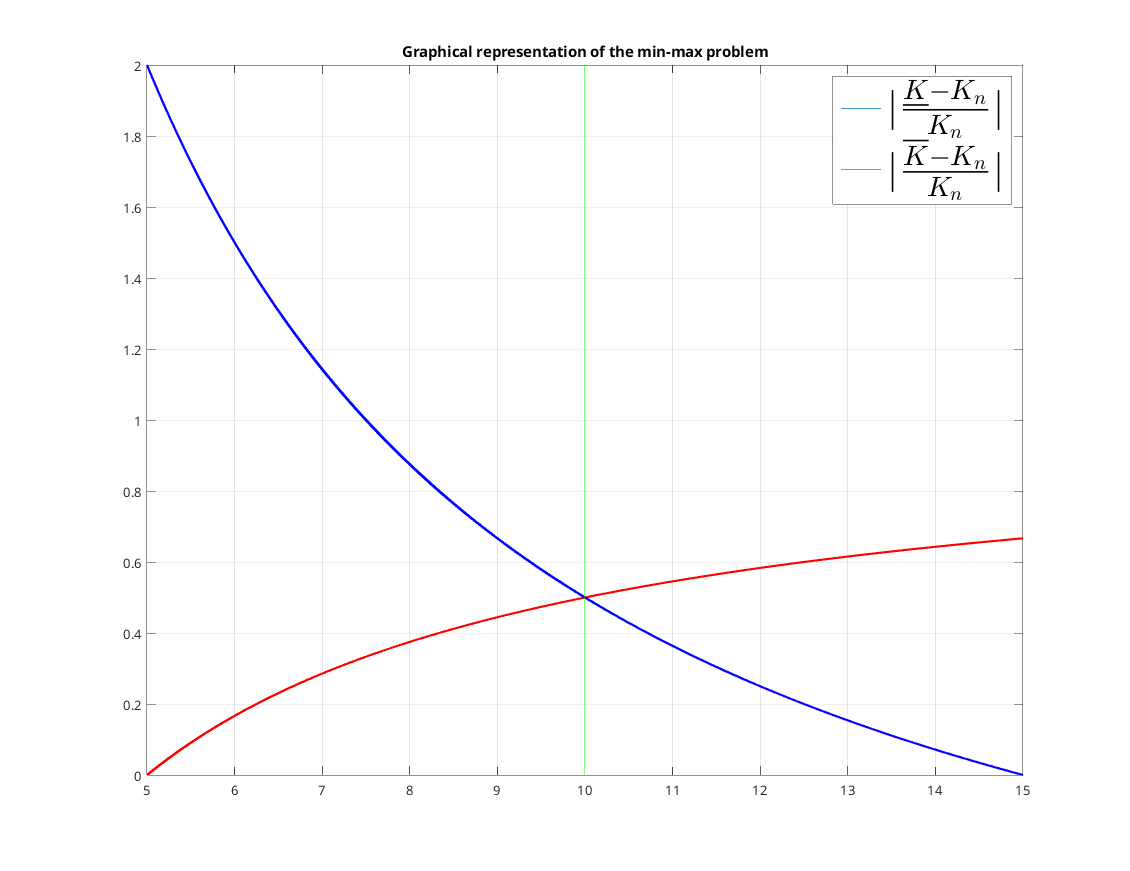
\includegraphics[width=0.5\textwidth]{minmax.png}
    \caption{Graphical representation of the minimization problem.}
\end{figure}

\begin{QandAbox}[Convervativeness Issue of unstructured uncertainty model sets]
Here, we remark that unstructured uncertainty model sets can only provide consvervative description of parametric uncertainties since, as shown in the previous exmaple, a complex function $\Delta(s)$ is used to account for the source of uncertainty, which is a real number. The unstructured uncertainty model set describes at each ferquency $\omega$ the uncertainty as a disk of radius $|W_u(j\omega)L_n(j\omega)|$ which is a conservative description of the actual uncertainty as shown in the following figure.
\end{QandAbox}
\begin{QandAbox}
\begin{figure}[H]
    \centering
    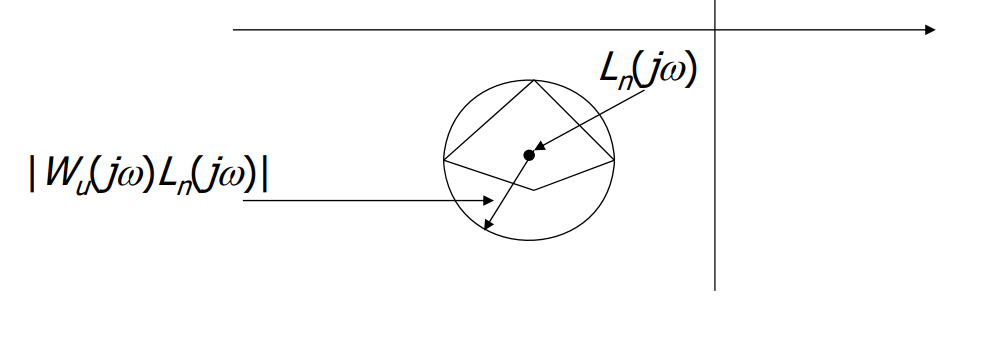
\includegraphics[width=0.75\textwidth]{conservative.png}
    \caption{Graphical representation of the conservetiveness issue of unstructured uncertainty model set.}
\end{figure}
\end{QandAbox}

\subsection{The inverse additive uncertainty model set}
The mathematical set of this kind of uncertainty model is as follows:
\[
M_m = \{G_p(s):\:G_p(s)\,=\,\frac{G_{pn}}{[1 + W_u(s)\Delta(s)G_{pn}(s)|},\,\|\Delta(s)\|_\infty\leq 1 \}
\]
\begin{figure}[H]
    \centering
    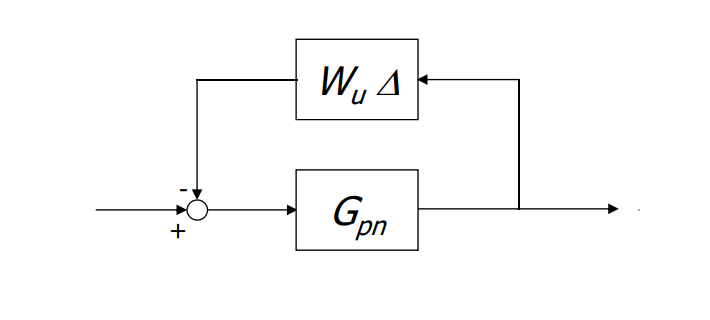
\includegraphics[width=0.5\textwidth]{inverse-additive.png}
    \caption{The block diagram description of inverse additive uncertainty}
\end{figure}

\subsubsection{Use cases:}
\begin{enumerate}
    \item \textbf{Uncertainty in System Poles:}\\
    \textbf{Scenario:} When the primary source of uncertainty affects the system’s poles rather than its zeros.\\
    \textbf{Why Inverse Additive:} Inverse additive uncertainty is effective in capturing changes in the denominator of the transfer function, which correspond to variations in the system poles.\\
    \textbf{Example:} A suspension system in a vehicle where damping ratios and natural frequencies are uncertain due to wear and environmental conditions.

    \item \textbf{Robustness to Controller Parameter Mismatch:}\\
    \textbf{Scenario:} When discrepancies between the designed and implemented controller parameters affect closed-loop behavior.\\
    \textbf{Why Inverse Additive:} Controller mismatch typically introduces pole shifts, which are well-represented by perturbations in the denominator.\\
    \textbf{Example:} A PID controller implemented with slightly incorrect gains, causing minor shifts in the closed-loop poles.

    \item \textbf{Dominance of Denominator Variations at Low Frequencies:}\\
    \textbf{Scenario:} When uncertainties in the system predominantly affect the low-frequency response due to variations in the denominator.\\
    \textbf{Why Inverse Additive:} At low frequencies, changes in the denominator significantly influence system behavior, making inverse additive uncertainty suitable.\\
    \textbf{Example:} A power grid experiencing load variations that alter the low-frequency impedance characteristics.

    \item \textbf{System Parameter Drift Over Time:}\\
    \textbf{Scenario:} When system parameters, such as time constants or damping ratios, drift over time due to aging or operational conditions.\\
    \textbf{Why Inverse Additive:} Parameter drifts primarily affect the poles of the transfer function, which are effectively modeled using inverse additive uncertainty.\\
    \textbf{Example:} An aging mechanical system where spring stiffness or damping properties degrade over time.

    \item \textbf{Uncertain Pole Placement in Control Design:}\\
    \textbf{Scenario:} When designing controllers for pole placement and the exact pole locations of the system are uncertain.\\
    \textbf{Why Inverse Additive:} This type of uncertainty directly represents variations in the desired pole locations.\\
    \textbf{Example:} A spacecraft attitude control system where uncertain moments of inertia introduce variability in the poles of the closed-loop transfer function.
\end{enumerate}



\subsection{The inverse multiplicative uncertainty model set}
The mathematical set of this kind of uncertainty model is as follows:
\[
M_m = \{G_p(s):\:G_p(s)\,=\,\frac{G_{pn}}{[1 + W_u(s)\Delta(s)|},\,\|\Delta(s)\|_\infty\leq 1 \}
\]
\begin{figure}[H]
    \centering
    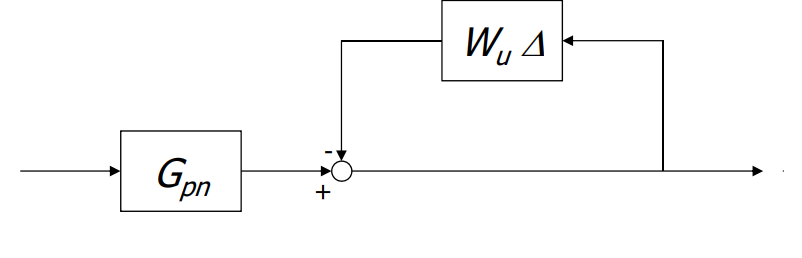
\includegraphics[width=0.5\textwidth]{inverse-multiplicative.png}
    \caption{The block diagram description of inverse additive uncertainty}
\end{figure}

\subsubsection{Use cases:}
\begin{enumerate}
    \item \textbf{Uncertainty in System Zeros:}\\
    \textbf{Scenario:} When the primary source of uncertainty affects the system’s zeros rather than its poles.\\
    \textbf{Why Inverse Multiplicative:} Inverse multiplicative uncertainty captures variations in the numerator of the transfer function, corresponding to changes in the system zeros.\\
    \textbf{Example:} An audio equalizer with varying zero locations due to inaccuracies in filter design.

    \item \textbf{Frequency-Dependent Uncertainty:}\\
    \textbf{Scenario:} When uncertainty is frequency-dependent and affects the system gain significantly at certain frequencies.\\
    \textbf{Why Inverse Multiplicative:} Frequency-dependent uncertainties are well-represented by scaling terms in the inverse multiplicative form.\\
    \textbf{Example:} A radio frequency amplifier with varying gain due to component aging or manufacturing tolerances.

    \item \textbf{Variations in System Gain:}\\
    \textbf{Scenario:} When uncertainties primarily influence the system gain, causing variations in the overall magnitude response.\\
    \textbf{Why Inverse Multiplicative:} Gain variations directly affect the numerator of the transfer function, aligning with the inverse multiplicative structure.\\
    \textbf{Example:} A hydraulic actuator where supply pressure fluctuations cause variability in the system's output gain.

    \item \textbf{Modeling Errors in High-Frequency Dynamics:}\\
    \textbf{Scenario:} When high-frequency dynamics introduce errors in the numerator of the transfer function.\\
    \textbf{Why Inverse Multiplicative:} Errors in high-frequency dynamics are often well-approximated by perturbations in the numerator, especially in systems where poles remain stable.\\
    \textbf{Example:} An industrial motor drive system with unmodeled high-frequency electrical effects.

    \item \textbf{System Behavior under Uncertain Input Conditions:}\\
    \textbf{Scenario:} When the system’s response is sensitive to input variations or disturbances, introducing uncertainty in the output.\\
    \textbf{Why Inverse Multiplicative:} The sensitivity of the system to input variations can often be modeled as changes in the numerator dynamics.\\
    \textbf{Example:} A robotic manipulator where input torque uncertainties affect the system’s trajectory.
\end{enumerate}

\textbf{From now on, we consider only multiplicative uncertainties for our systems.}

In order to chose the weight function, a practical way is to plot different members of the family, 10 sample at least for each parameter, and then consider $W_u$ to be a transfer function passing the maximum of all the magnitudes, shown in the following figure.
\begin{figure}[H]
    \centering
    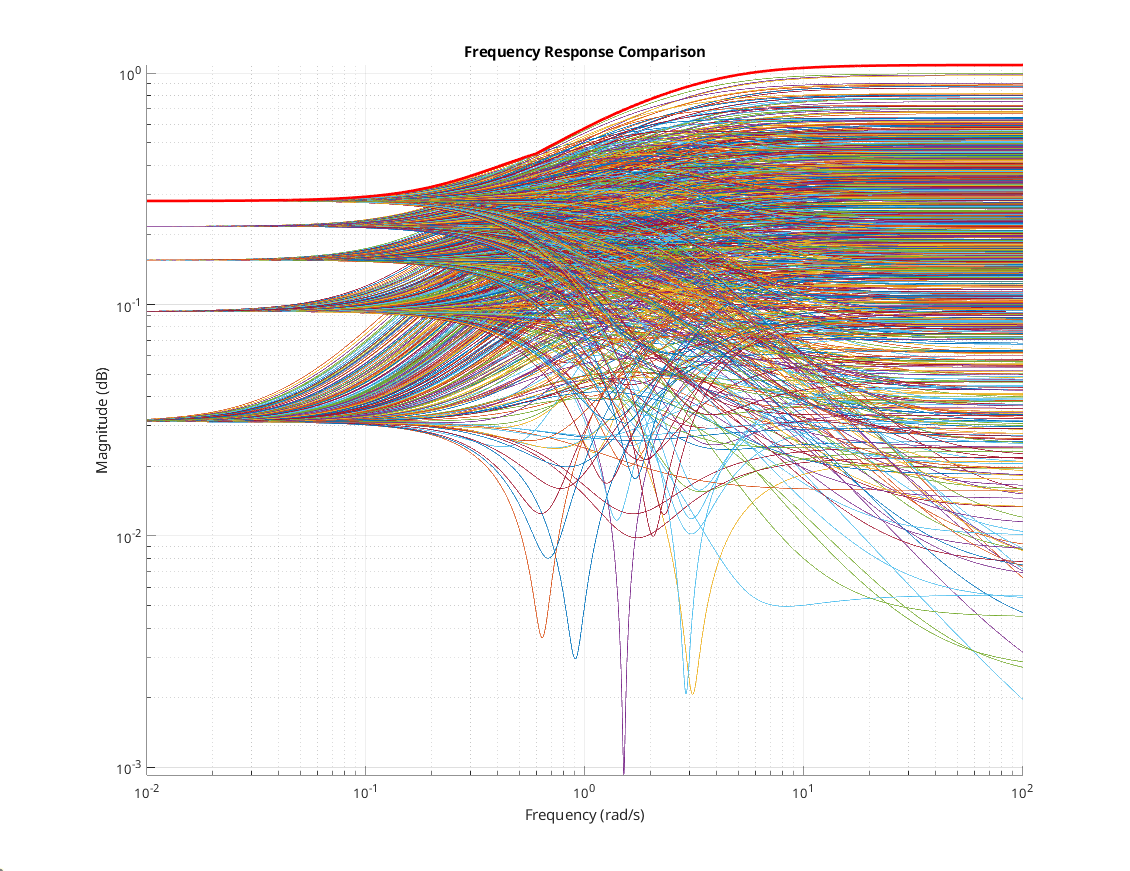
\includegraphics[width=1\textwidth]{uncertainty-weighting.png}
    \caption{The bold red plot is the transfer function that satisfies the inequality considered for $\delta$}
\end{figure}
FOR THE CODE, CHECK LABORATORY 06

The fitting tool, 'magfit()' command in matlab, used for finding $W_u$, usually returns a strictly proper transfer function, while it is recommended to model the uncertainty as fit as possible to the maximum value of the data, so in some cases, we may need to remove one or two zeros at this end. In the following figure, the blue dashed line is the output of the fitting tool, and the black dashed line is the modified weighting function.

\begin{figure}[H]
    \centering
    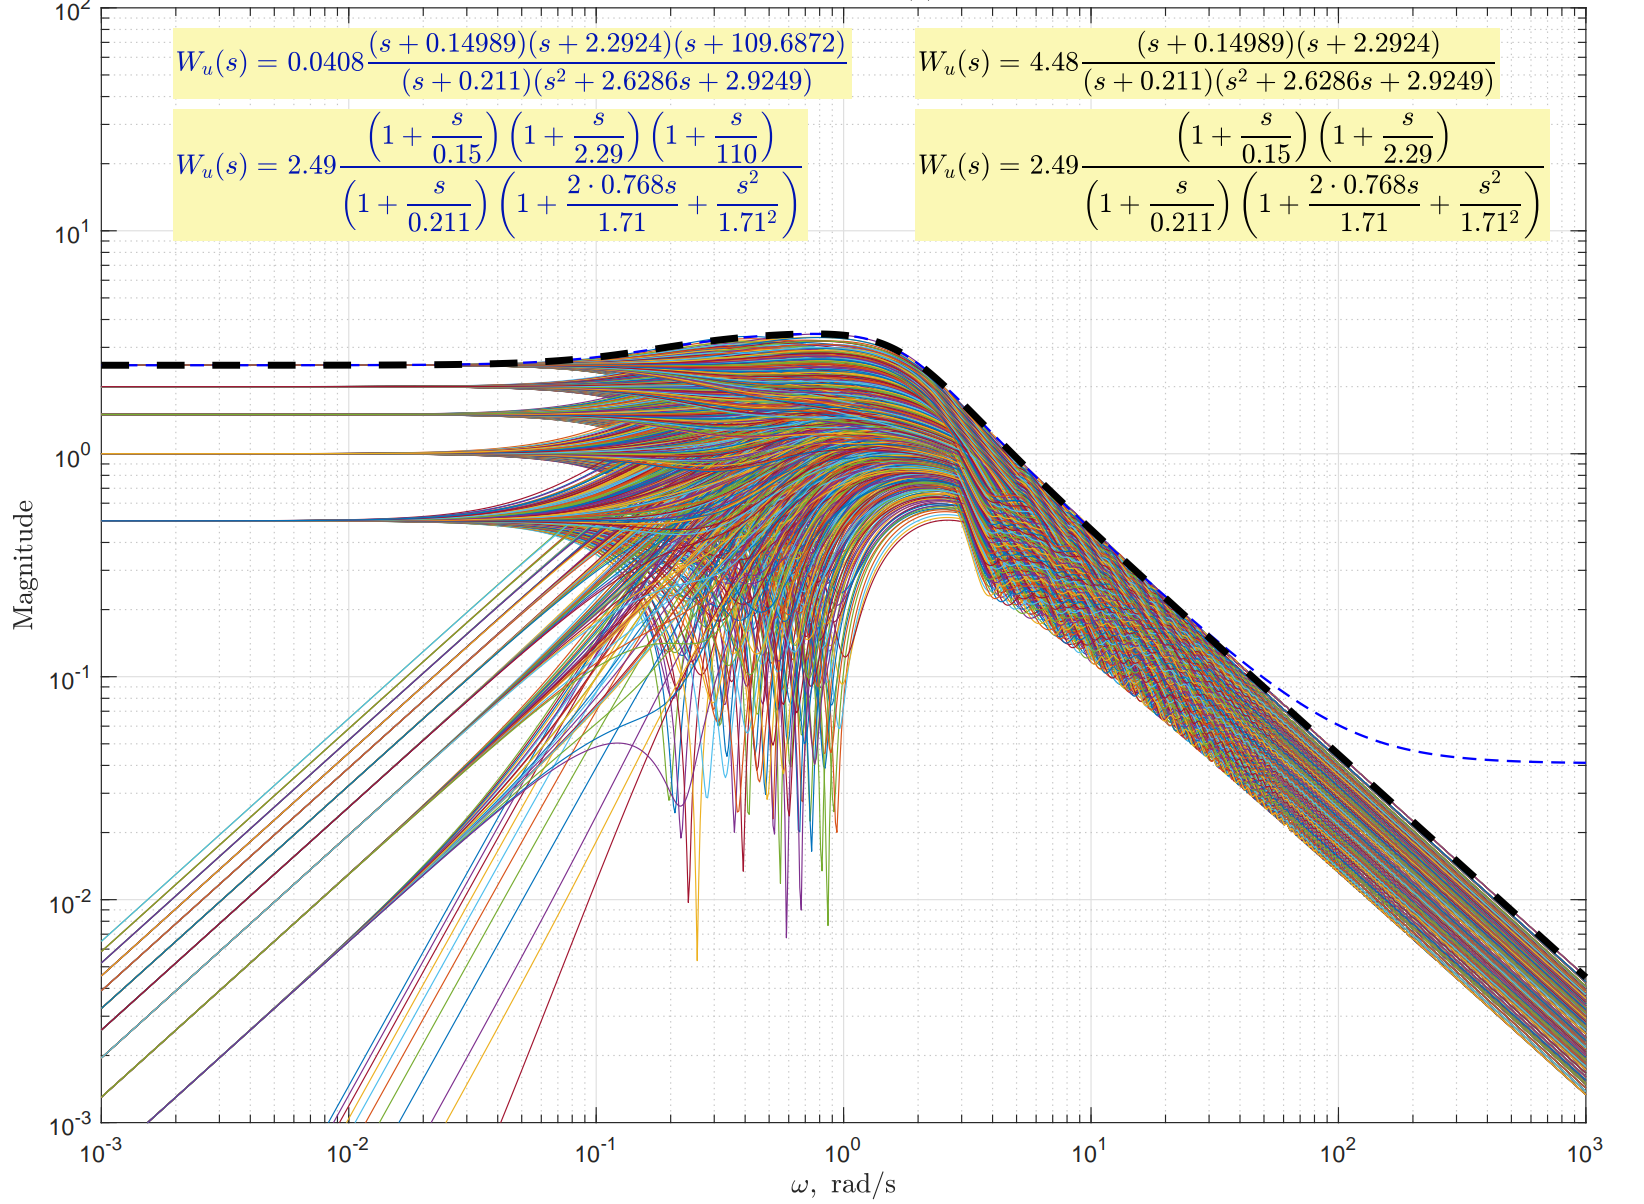
\includegraphics[width=1\textwidth]{Wu-proper.png}
    \caption{The plot of the uncertainties for the models of the model set and the corresponding strictly proper and proper $W_u$.}
\end{figure}

\begin{factbox}
In the low frequency range and middle frequency range, we should have $W_u$ pretty tight, but it can be loose in the high frequency range, because $T$ is a low pass transfer function and at high frequnecies its value is low. Nonetheless, it is recommended to make $W_u$ everywhere as tight as possible.\\
Another note that try to make the degree of the weighting function as low as possible. By doing so, the degree of the resultant controller is going to be low as well.
\end{factbox}

\begin{QandAbox}
In $\mu$ analysis, we can use linear algebra tools to obtain an upper and lower bounds for parameter uncertainties. As a result, for a given performance, how precise should the description of the plant be.
\end{QandAbox}
\section{Robust stability}
We aim at studying the stability of this feedback control system under the assumption that $G_p$ is an uncertain system describe by a given uncertainty model set. In particular, as it was mentioned, we assume, here, that $G_p$ belogns to a multiplicative uncertainty model set $M_m$.

\subsubsection{Definition (Robust Stability)}
The feedback system in the figure is \textbf{robustly stable} if and only if it is internally stable for each $G_p$ which belongs to $M_m$.
\[
M_m = \{G_p(s): G_p(s) = G_{pn}[1+W_u(s)\Delta(s)],\|\Delta(s)\|_\infty \leq 1\}
\]
\begin{figure}[H]
    \centering
    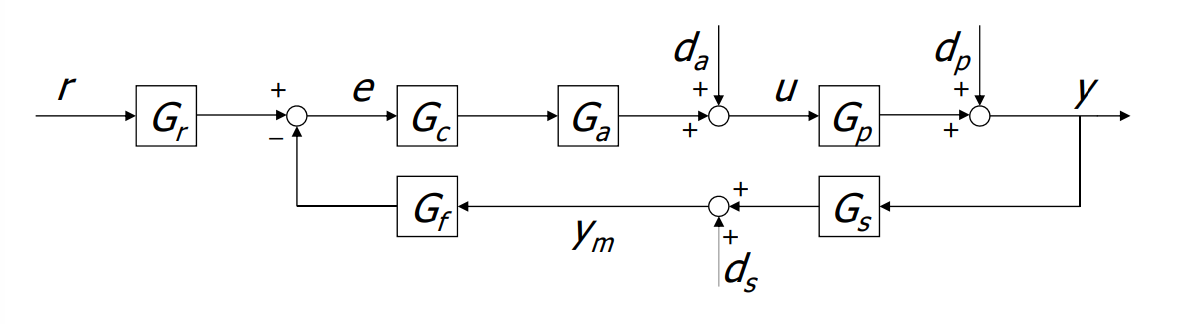
\includegraphics[width=1\textwidth]{block-scheme.png}
    \caption{The block diagram scheme of the feedback control system.}
\end{figure}

\subsubsection{Result (Robust Stability and multiplicative uncertainty)}
Assume that $G_p$ belogns to $M_m$, and assume that the feedback control system is stable when the nominal model $G_{pn}$ is considered as the model of the plant. The feedback system is \textbf{robustly stable} if and only if the following condition is satisfied:
\[
\|W_uT_n\|_\infty < 1
\]

where $Tn$ is the nominal complementary sensitivity function:d
\[
T_n = \frac{L_n}{1 + L_n}
\]
Where $L_n$ is the loop shaping function made by $G_{pn}$.


\subsection{sketch of the proof}
Let us define the nominal loop function as $L_n$. Since the feedback control system is stable for $G_p = G_{pn}$ by hypothesis, we know from the Nyquist criterion that the Nyquist plot of $L_n$ does not pass through the point -1 and its number of counter-clockwise encirclements equals the number of the poles of $L_n$ with positive real part.

As to the uncertain system, from the Nyquist theorem, we know that the feedback control system is robustly stable for $G_p = G_{pn}(1 + W_u\Delta)$ if and only if the Nyquist plot of $L = L_n(1 + W_u\Delta)$ does not cross the point $-1$ and its number of counter-clockwise encirlements equals the number of poles of $L_n$ with positive real part. we have that:
\[
L = L_n(1+W_u\Delta) \Rightarrow L-L_n = L_n W_u\Delta
\]
where
\[
\|\Delta(s)\|_\infty \leq 1 \Rightarrow |\Delta(j\omega)|\leq 1 \:\:\:\:\: \forall \omega
\]

\begin{figure}[H]
    \centering
    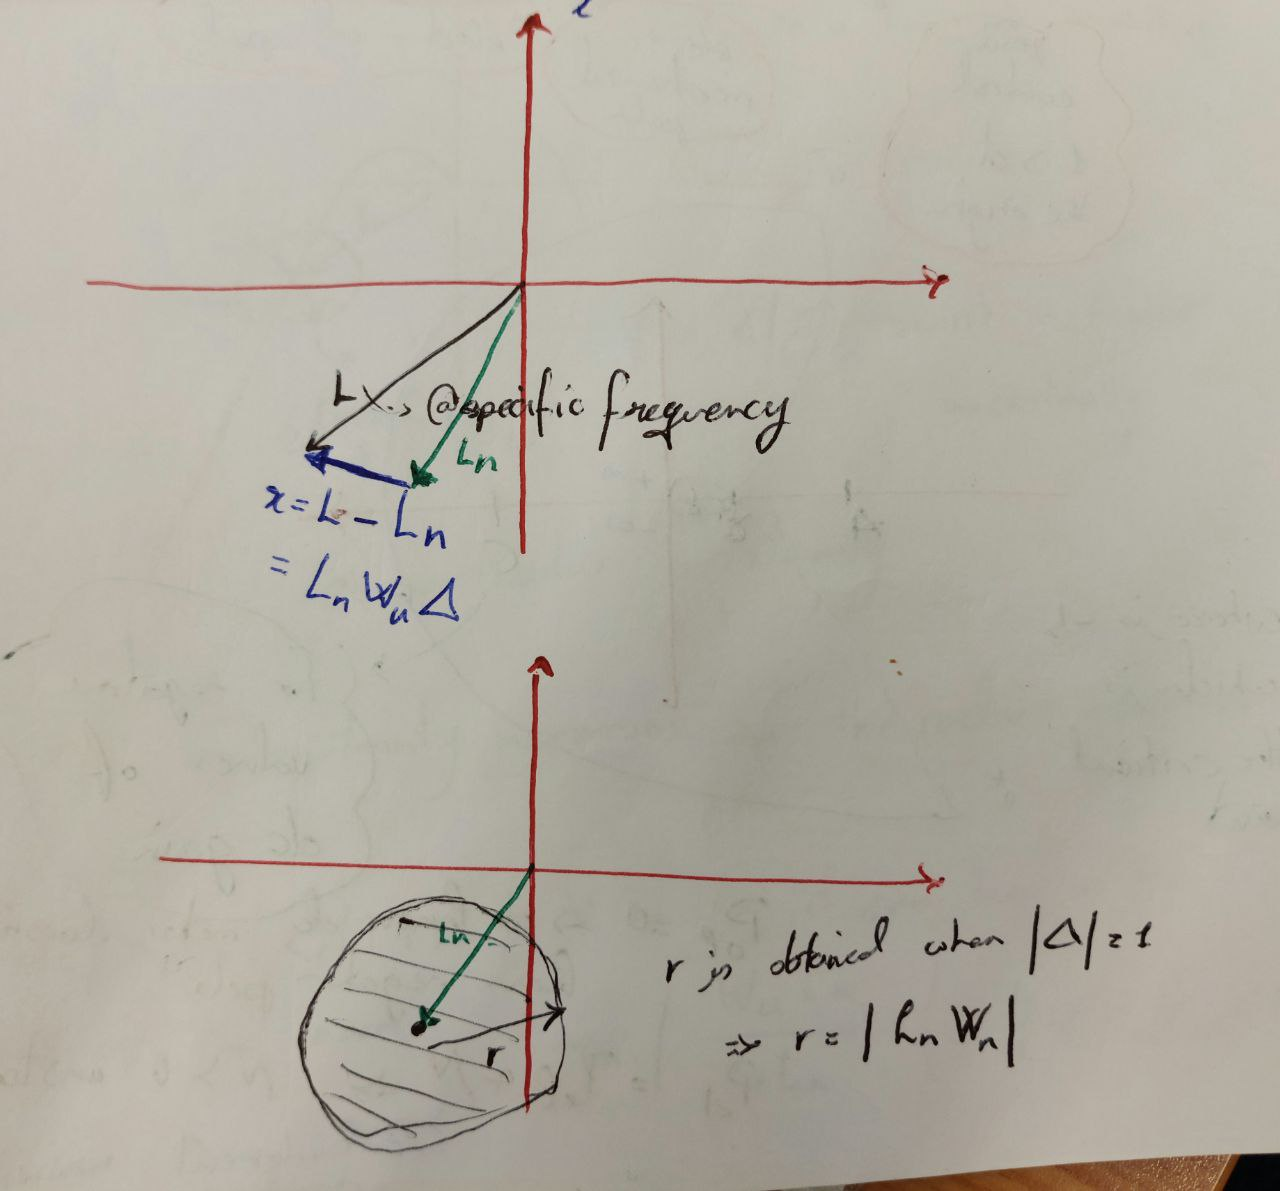
\includegraphics[width=0.6\textwidth]{L-Ln.jpg}
    \caption{Graphical representation of $L-L_n$ on the complex plane for a given frequency}
\end{figure}

\begin{figure}[H]
    \centering
    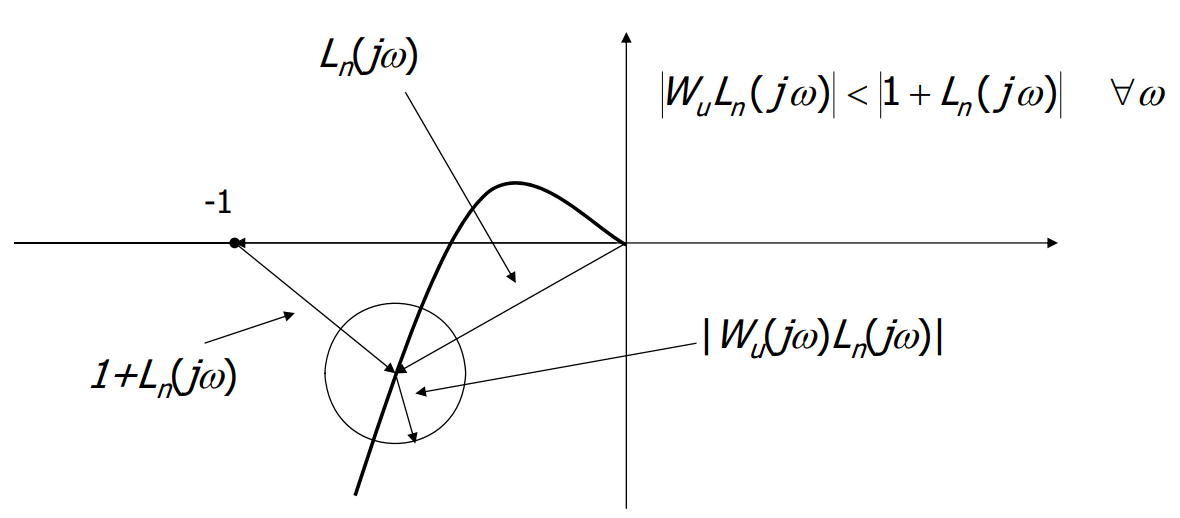
\includegraphics[width=0.75\textwidth]{robust-stability.png}
    \caption{The representation of the uncertainty disk.}
\end{figure}
It can be seen that if uncertainty increases, the circle approaches -1.
Since the uncertainty must not change the number of encirclements, the following condition for robust stability is obtained:
\[
|W_uL_n(j\omega)|\leq|1+L_n(j\omega)| \:\:\:\:\: \forall \omega
\]

which is equivalent to:
\[
\sup\limits_{\omega}|\frac{W_uL_n(j\omega)}{1+L_n(j\omega)}|=\|W_uT_n\|_\infty \leq 1
\]

\begin{example}[Example for Nyquist theorem]
Consider the transfer function of a feedback control system for position control of an electrical motor. The qualitative Nyquist plot of the loop function is shown in the following figure.
\begin{figure}[H]
    \centering
    \includegraphics[width=0.75\textwidth]{nyquist.jpg}
    \caption{Qualitative nyquist plot of an electric motor with position control.}
\end{figure}
Based on whether -1 is at the points A, B, or C, the stability characteristic of the nominal plant changes.\\
(A) $N = 0$, the nominal system is \textbf{stable}\\
(B) $N = 2$, the nominal system is \textbf{unstable} with two positive poles.\\
(C) $N = 1$ the system is unstable with one positive pole.
\end{example}
Robust statability condition for the remaining three uncertainty model sets can be obtained in a similar way. The following result summarizes the robust stability conditions for the four uncertainty model set considered. Note that $S_n = 1 - T_n$.
\begin{figure}[H]
    \centering
    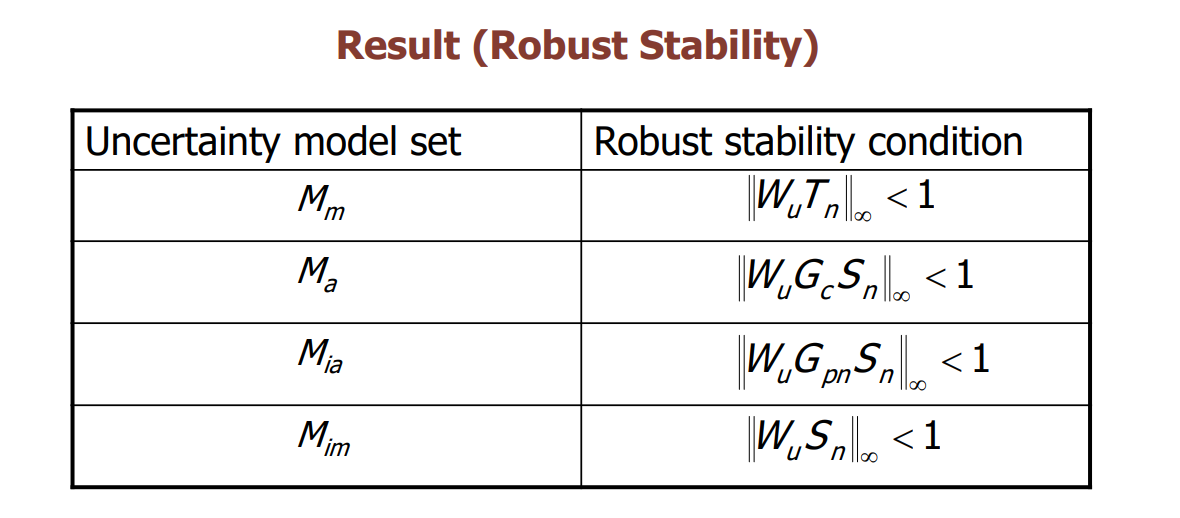
\includegraphics[width=0.75\textwidth]{robust-stability-results.png}
    \caption{The robust stability results for the four unstructured uncertainty models.}
    \end{figure}

\begin{QandAbox}[Very important point to be considered]
Pay attention that due to the conservativeness issue of unstructured uncertainty model sets. If the disk does not surpasses -1 for all the frequencies. We are sure that the system is robustly stable. However, \textbf{if for some frequencies the disk surpasses, it does not mean that the system is for sure robustly unstable.}\\

    Consider the following transfer function with the gain K being uncertain.
\[
G_{pn}(s) = \frac{K}{s(1+\frac{s}{p_1})(1+\frac{s}{p_2})}
\] 
In this case, the real uncertainty is on the length of L , while the multiplicative unstructured uncertainty introduces a disk at each frequency. which is not true. This disk may crosses -1 for some frequencies while the true system is robustly stable.

\begin{figure}[H]
    \centering
    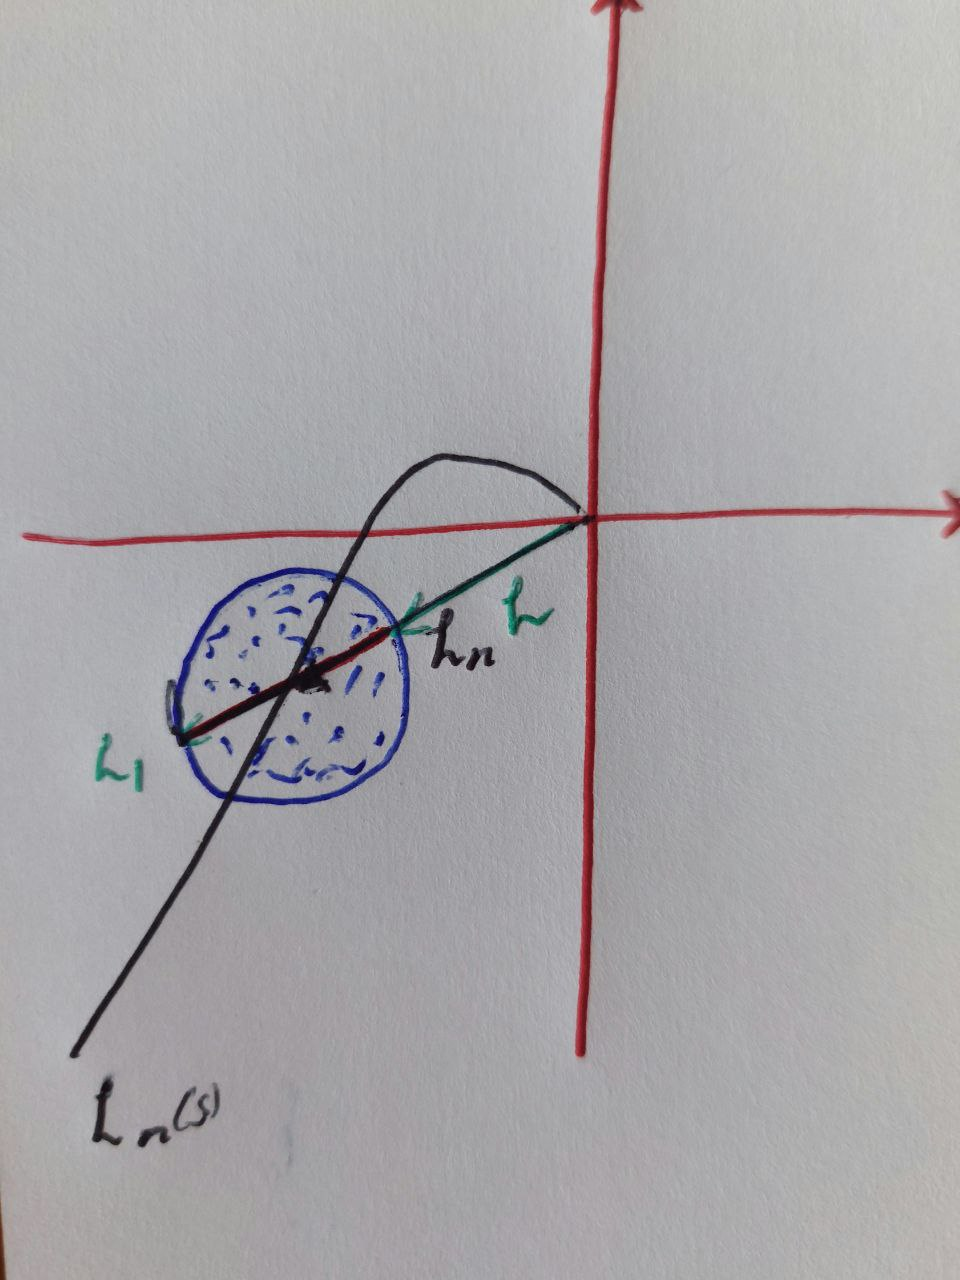
\includegraphics[width=0.5\textwidth]{true-uncertainty.jpg}
    \caption{The qualitative polar plot of the abovementioned transfer function.}
\end{figure}
   

\end{QandAbox}
\section{Nominal performance}
\begin{factbox}[professor's quote]
Always check the performance through time-domain simulation. The reason is that the translation of the requirements in frequency domain is not exact, we used the 2nd-order prototype system guidline, which does not tend to be the exact description of the system. \\
Another reason for checking the real-time performance is the conservativeness issue of unstructured uncertainty modelling.
\end{factbox}

\begin{QandAbox}[Performance limitatioons]
The crossover frequency should be larger that half of the real part of a system with non-minimum pole and should smaller than that for a system with a non-minimum zero. For further reading, take a look at the main source book pages 112 to 115.
\end{QandAbox}

Here, we recall the nominal performance conditions (i.e. performance conditions in the uncertainty-free case) derived previously. Performance requirements affecting the sensitivity function leads to the following condition;
\[
\|W_SS_n\|_\infty \leq 1 \Leftrightarrow |1 + L_n(j\omega)| > |W_s(j\omega)| \forall \omega
\]
while performance requirements affecting the complementary sensitivity function are translated into:
\[
\|W_TT_n\|_\infty \leq 1 
\]

\begin{figure}[H]
    \centering
    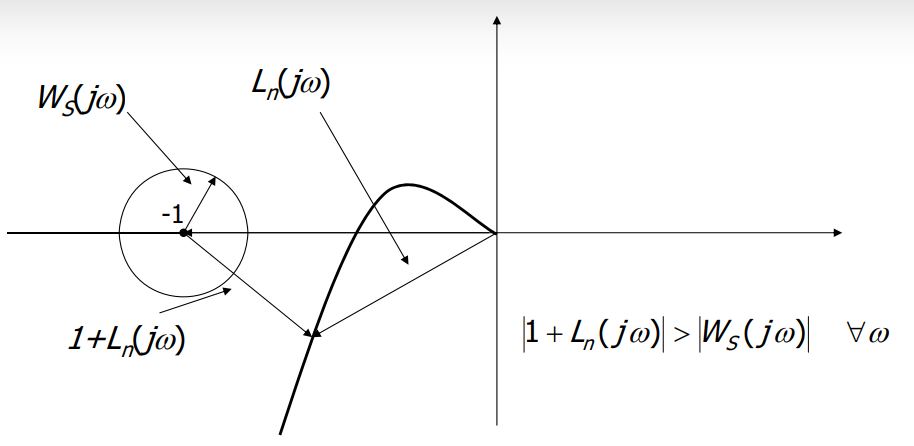
\includegraphics[width=0.75\textwidth]{nominal-performance.png}
    \caption{The qualitative polar plot showing nominal performance requirement on sensitivity.}
\end{figure}

Regarding the Bode plot, $W_S$ and $S_n$ must be exact when $s$ tends to zero and at the pick, while for the transient this is not the case.


\begin{figure}[H]
    \centering
    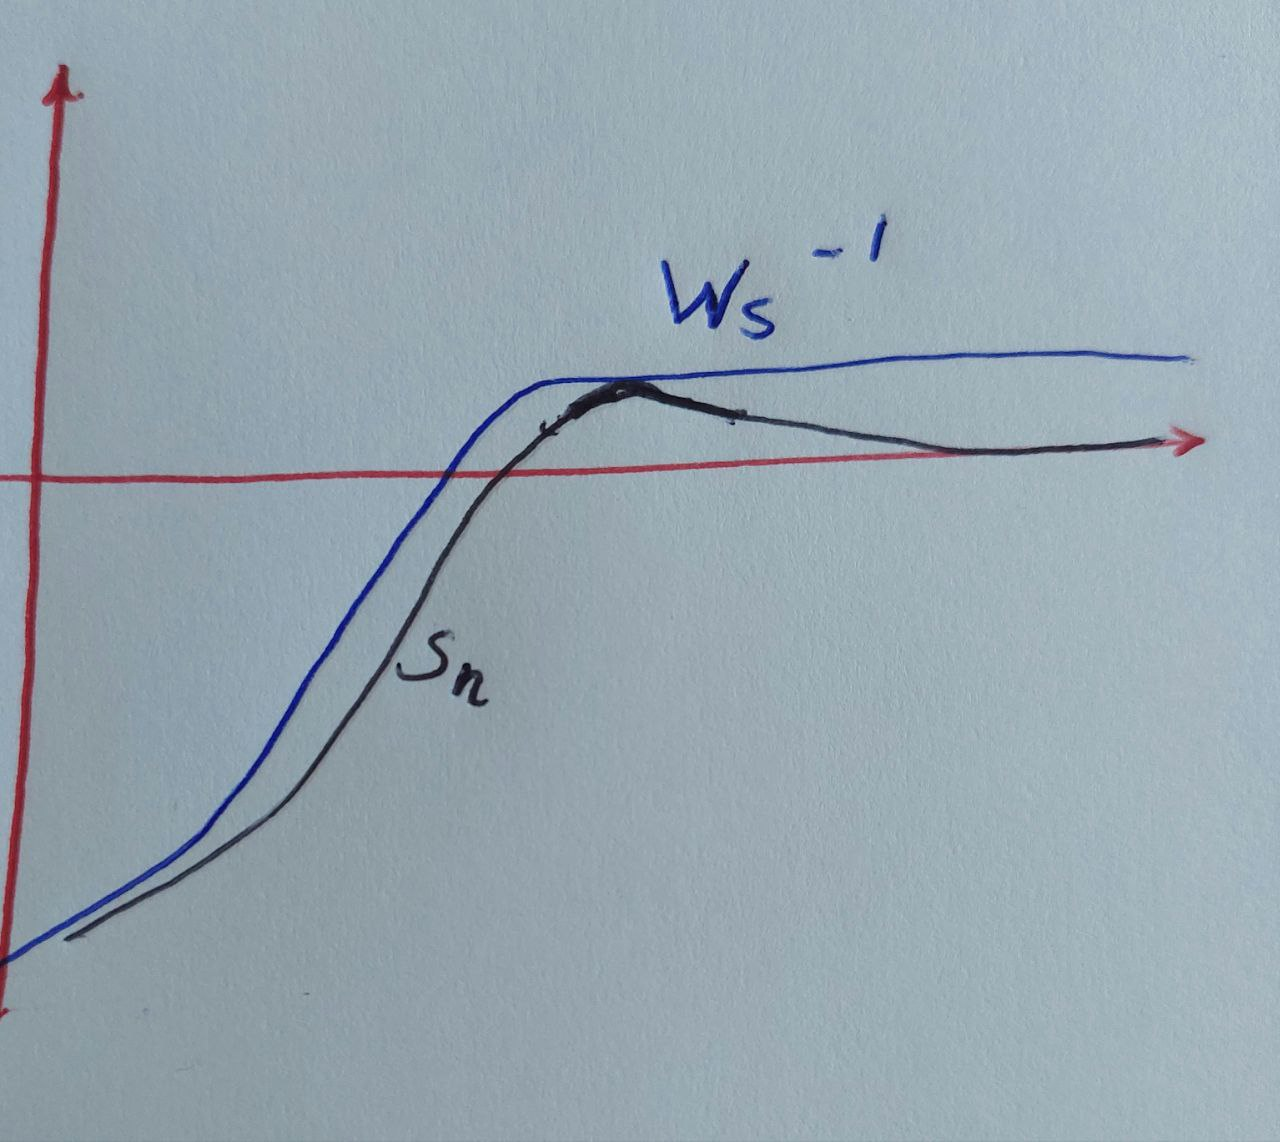
\includegraphics[width=0.5\textwidth]{nominal-performance-1.jpg}
    \caption{The nominal performance}
\end{figure}


\section{Robust performance}
\subsection{Definition}
The feedback system guarantees robust performance if and only if the performance requirements are satisfied for each $G_p$ which belongs to the given uncertainty model set.

Here, we consider the particular case where: 
\begin{itemize}
    \item performance requirements affect only the sensitivity function
    \item uncertainty is described by menas of a multiplicative model set $M_m$
\end{itemize}

The following result provides necessary and sufficient conditions for robust performance under such assumptions.

\subsection{Result}
The feedback system guarantees robust performance if and ony if the following condition is satisfied:
\[
\|W_SS_n||+|W_uT_n|\|_\infty < 1
\]
\subsection{Sketch of the proof}
By definition, the feedback system guarantees robust performance if and only if:
\[
\|W_SS\|_\infty < 1
\]
where
\[
S = \frac{1}{1+L_n(1+W_u\Delta)}
\]
thus, we can write the following robust performance condition:
\[
\|\frac{W_S}{1+L_n(1+W_u\Delta)}\|_\infty < 1
\]

which, being $L = L_n(1+W_u\Delta)$, can be equivalently written as:
\[
|1+L(j\omega)| > |W_S(k\omega)| \forall \omega
\]

This last condition means that at each frequency the loop function of th euncertaint system must stay outside the circle of radius $|W_S(j\omega)|$ centered at -1. \\
Now, let us consider the following relation straightforwardly derived from the definition of multiplicative uncertainty model set on the loop transfer function:
\[
|L(j\omega)-L_n/(j\omega)| \leq |W_u(j\omega)L_n(j\omega)| \:\:\:\:  \forall \omega
\]


From the following figure, it is clear that the feedback system guarantees robust performance if and only if the two disks do not overlap.


\begin{figure}[H]
    \centering
    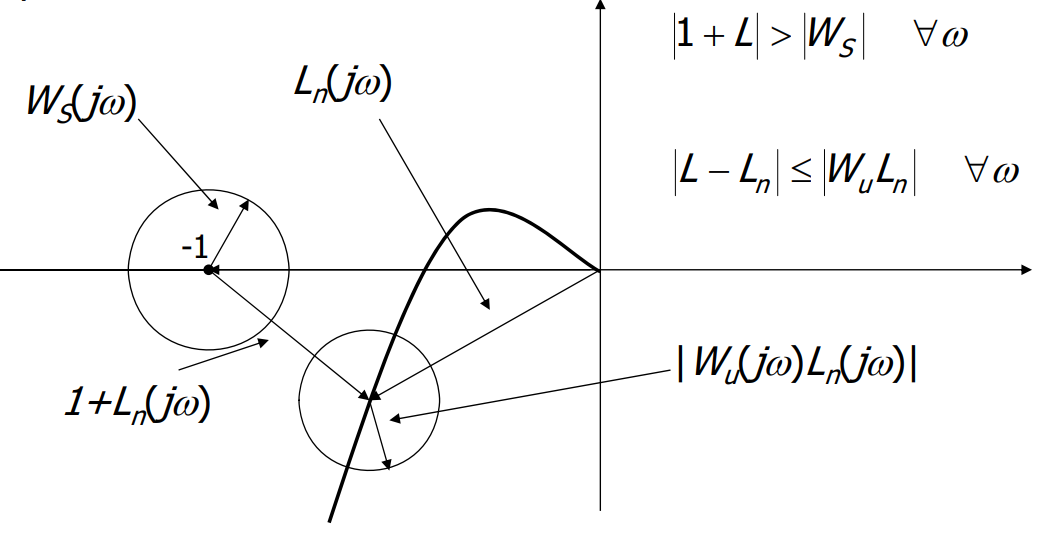
\includegraphics[width=0.5\textwidth]{robust-performance.png}
    \caption{The graphical reasoning for robust performance}
\end{figure}


The condition to avoid overlapping of of the two disks can be formally written as:
\[
\begin{array}{c}
|W_S|+|W_uL_n|<|1+L_n| \:\:\:\forall \omega \Leftrightarrow
|\frac{W_S}{1+L_n}|+|\frac{W_uL_n}{1+ L_n}|<1  \:\:\:\forall \omega
\\
\Leftrightarrow
\||W_SS_n|+|W_uT_n|\|_\infty <1
\end{array}
\]

which is the condition stated in the result.

\begin{QandAbox}[Some comments]
I) If $W_u$ in the case of unstructured uncertainty crosses $W_{Tn}$, we cannot conclude that robust stability is not satisfied \textbf{becaues of the conservativeness issue} which was discussed. However, if they don't cross, we can be sure that the system is robustly stable, putting for the same argument.\\

II) Since T is a low pass filter, the effect of high-frequency poles and zeros is going to be reduces. So it can be seen that even if we have high-frequency uncertainties  in $W_u$, at high frequencies, the multiplication of $W_uT_n$ is going to be small.
\end{QandAbox}

\begin{factbox}[Curiosity]
?? In $\mu$-analysis, we may be able to use linear algebra tools to obtain upper-bounds and lower-bounds for the parameter uncertainties in order to guarantee certain performance requirements. ?? If this is the case, we can use it to design the identification problem much easier.
\end{factbox}











